\documentclass[conference]{IEEEtran}

% --- Essential Packages ---
\usepackage[utf8]{inputenc}
\usepackage{amsmath,amssymb,amsfonts}
\usepackage{graphicx}
\usepackage{booktabs}
\usepackage{multirow}
\usepackage{array}
\usepackage{tabularx}
\usepackage{algorithm}
\usepackage{algorithmic}
\usepackage{cite}
\usepackage{url}
\usepackage{microtype}
\usepackage{tikz}
\usetikzlibrary{shapes.geometric, arrows.meta, positioning}
\usepackage{xcolor}

\begin{document}

% --- Paper Title ---
\title{Decoupled Secondary Row Buffer Architecture for Processing-In-Memory Acceleration of Large Language Model Workloads}

% --- Author Block ---
\author{
    \IEEEauthorblockN{Anirudh Bhardwaj}
    \IEEEauthorblockA{\textit{Department of Computer Science and Engineering} \\
    \textit{Indian Institute of Technology Guwahati}\\
    Guwahati, Assam, India -- 781039 \\
    Email: anirudh.bhardwaj@iitg.ac.in}
}

\maketitle

% --- Abstract ---
\begin{abstract}
Serving autoregressive Large Language Models (LLMs) is fundamentally bottlenecked by off-chip memory traffic across physical channels---the well-known \textit{Memory Wall}. Through hardware profiling of modern open-source LLM inference engines (\texttt{llama.cpp}) using NVIDIA Nsight Systems, Nsight Compute, and Valgrind Cachegrind, we reveal that matrix multiplication routines account for over $89\%$ of total execution latency. Crucially, the token generation (decode) phase is dominated by Matrix-Vector Multiplication (GEMV), which exhibits a strictly constant operational intensity of $I_{\text{op}} = 0.5$~FLOP/byte. This forces catastrophic Last-Level Cache (LLC) thrashing ($>95\%$ miss rates) and caps CPU/GPU core utilization at under $5\%$. While Processing-in-Memory (PIM) offers an intuitive remedy by leveraging internal bank bitline bandwidth, commodity DRAM architectures suffer from destructive row-conflict stalls whenever multi-operand arithmetic is executed within a single bank. 

In this work, we propose, model, and evaluate a PIM-DRAM microarchitecture featuring \textbf{Decoupled Secondary Row Buffers (SRB)}. By augmenting each bank with an 8-row SRAM buffer ($64$~KB per bank, matching UPMEM WRAM capacity) and an atomic auto-precharging command (\texttt{PIM\_ACT\_SRB}), our design isolates in-memory arithmetic from primary sense amplifiers, eliminating primary bank row conflicts entirely. We evaluate this architecture using a cycle-accurate timing simulator across 128 autonomous banks against both single-threaded naive and multi-threaded AVX2+FMA OpenMP CPU baselines. For memory-choked GEMV workloads ($N \le 8192$), our architecture achieves up to \textbf{$1,452\times$} speedup over the naive baseline and up to \textbf{$346\times$} over the steady-state AVX2 multi-threaded CPU baseline (using 16-wide Vector ALUs), while 8-wide SIMD delivers up to \textbf{$766\times$ / $186\times$} speedup. On compute-bound GEMM workloads ($N \le 8192$), PIM maintains $O(N^3)$ computational regularity, achieving up to \textbf{$434\times$} speedup over naive CPU execution and \textbf{$29.9\times\text{--}33.6\times$} over steady-state optimized multi-core CPU execution.
\end{abstract}

\begin{IEEEkeywords}
Processing-in-Memory (PIM), Large Language Models (LLMs), Secondary Row Buffers (SRB), DRAM Microarchitecture, Roofline Model, GEMV Acceleration, Memory Wall.
\end{IEEEkeywords}

% -------------------------------------------------------------------------
\section{Introduction}
\label{sec:intro}
% -------------------------------------------------------------------------
Autoregressive Transformer-based Large Language Models (LLMs)~\cite{touvron2023llama, brown2020language} have emerged as the foundational workload of modern artificial intelligence. However, serving foundational models with billions of parameters exposes the fundamental limitations of traditional Von Neumann architectures. While silicon compute capability has expanded rapidly, off-chip memory bandwidth has scaled at a much slower pace, resulting in the classical \textit{Memory Wall}~\cite{mutlu2019processing}.

Inference in Transformer models exhibits two sharply divergent computational regimes across its operational lifecycle:
\begin{enumerate}
    \item \textbf{Prompt Prefill Phase (GEMM):} The initial user prompt is processed in parallel using General Matrix-Matrix Multiplication ($C = A \cdot B$). With an algorithmic complexity of $O(N^3)$ operations over $O(N^2)$ data elements, GEMM features high operational intensity ($I_{\text{op}} \approx N/2$~FLOP/byte), enabling CPU and GPU cache hierarchies to effectively reuse matrix tiles.
    \item \textbf{Token Generation / Decode Phase (GEMV):} Tokens are generated autoregressively one by one. In every iteration, the newly predicted token vector ($1 \times N$) must be multiplied against the entire weight matrix ($N \times N$) of each layer via General Matrix-Vector Multiplication ($y = A \cdot x$).
\end{enumerate}

For dimension $N$, GEMV performs $2N^2$ floating-point operations over $4N^2$ bytes of single-precision matrix weights:
\begin{equation}
    I_{\text{op}}^{\text{GEMV}} = \frac{2N^2\text{ FLOPs}}{4N^2\text{ bytes}} = 0.5\text{ FLOPs/byte}
    \label{eq:gemv_intensity}
\end{equation}

Equation~(\ref{eq:gemv_intensity}) underscores a catastrophic architectural reality: \textit{GEMV operational intensity is constant and independent of matrix dimension $N$}. Every single model parameter must be transferred across the physical memory bus to execute exactly one multiply-accumulate (MAC) operation before being discarded. On a commodity DDR4 channel with $30$~GB/s peak bandwidth, theoretical throughput is strictly capped at $30 \times 0.5 = 15$~GFLOPS, leaving hundreds of compute cores idling on memory stalls.

Processing-in-Memory (PIM) circumvents the external bus bottleneck by placing arithmetic units directly inside or adjacent to DRAM banks, tapping into terabytes-per-second of internal bitline bandwidth~\cite{mutlu2020modern, lee2021hardware}. However, integrating compute logic inside conventional DRAM banks introduces a critical microarchitectural conflict: standard DRAM banks feature only a \textit{single} sense amplifier row buffer. Performing arithmetic operations between two distinct rows ($Row_A$ and $Row_B$) within the same bank causes continuous row buffer conflicts, forcing repeated precharge ($t_{RP}$) and activation ($t_{RCD}$) cycles that cripple throughput.

In this paper, we present the design and empirical evaluation of a \textbf{Decoupled Secondary Row Buffer (SRB)} PIM architecture that resolves the internal row-conflict bottleneck. By isolating compute logic from primary bitlines through multi-slot SRAM buffering and atomic micro-commands, our architecture enables continuous, conflict-free in-DRAM matrix execution. The remainder of this paper details empirical profiling motivation (Section~\ref{sec:profiling}), the SRB-PIM microarchitecture and data layout (Section~\ref{sec:arch}), our cycle-accurate simulation methodology (Section~\ref{sec:methodology}), experimental evaluation (Section~\ref{sec:evaluation}), related work (Section~\ref{sec:related}), architectural trade-offs and limitations (Section~\ref{sec:scope}), and conclusions (Section~\ref{sec:conclusion}).

% -------------------------------------------------------------------------
\section{Empirical Profiling and Motivation}
\label{sec:profiling}
% -------------------------------------------------------------------------

\subsection{Profiling llama.cpp on Physical Hardware}
To ground our architectural design in empirical evidence, we characterized the execution profile of modern LLM inference. We profiled the \texttt{llama.cpp} inference engine running LLaMA architectures using NVIDIA Nsight Systems (\texttt{nsys}), NVIDIA Nsight Compute (\texttt{ncu}), and Valgrind Cachegrind.

\begin{figure}[t]
\centering
\resizebox{\columnwidth}{!}{%
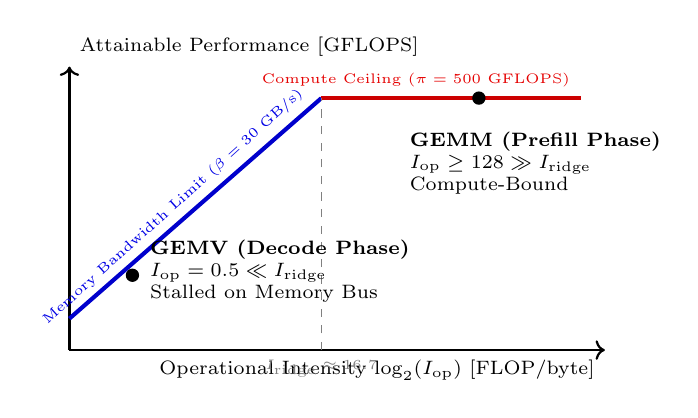
\begin{tikzpicture}
    \begin{scope}[font=\footnotesize]
        % Axes
        \draw[->, thick] (0,0) -- (6.8,0) node[below left, font=\scriptsize] {Operational Intensity $\log_2(I_{\text{op}})$ [FLOP/byte]};
        \draw[->, thick] (0,0) -- (0,3.6) node[above right, font=\scriptsize] {Attainable Performance [GFLOPS]};
        
        % Memory Bandwidth line
        \draw[line width=1.5pt, blue!80!black] (0,0.4) -- (3.2,3.2) node[above left, rotate=42, font=\tiny, text=blue!90!black] {Memory Bandwidth Limit ($\beta = 30$ GB/s)};
        % Compute roof
        \draw[line width=1.5pt, red!80!black] (3.2,3.2) -- (6.5,3.2) node[above left, font=\tiny, text=red!90!black] {Compute Ceiling ($\pi = 500$ GFLOPS)};
        
        % Ridge point
        \draw[dashed, gray] (3.2,0) -- (3.2,3.2);
        \node[below, font=\tiny, gray] at (3.2,0) {$I_{\text{ridge}} \approx 16.7$};
        
        % GEMV Point
        \filldraw[black] (0.8,0.95) circle (2.2pt);
        \node[right, font=\scriptsize, align=left] at (0.9,1.0) {\textbf{GEMV (Decode Phase)}\\$I_{\text{op}} = 0.5 \ll I_{\text{ridge}}$\\Stalled on Memory Bus};
        
        % GEMM Point
        \filldraw[black] (5.2,3.2) circle (2.2pt);
        \node[below right, font=\scriptsize, align=left] at (4.2,2.9) {\textbf{GEMM (Prefill Phase)}\\$I_{\text{op}} \ge 128 \gg I_{\text{ridge}}$\\Compute-Bound};
    \end{scope}
\end{tikzpicture}%
}
\caption{Roofline model illustrating the operational contrast between compute-bound GEMM (Prefill) and strictly memory-bandwidth-bound GEMV (Decode).}
\label{fig:roofline}
\end{figure}

The profiling revealed three critical insights:
\begin{enumerate}
    \item \textbf{Dominance of Matrix Arithmetic:} Quantized matrix kernels (\texttt{mul\_mat\_q} for prefill and \texttt{mul\_mat\_vec\_q} for decode) consistently consume $\approx 89\%$ of total execution latency. All non-linear operations (Softmax, RMSNorm, RoPE embedding) together consume less than $11\%$.
    \item \textbf{Catastrophic Cache Thrashing:} During token generation, Nsight Compute captured an L2 cache miss rate exceeding $95\%$. Because the model weight matrices vastly exceed Last-Level Cache (LLC) capacity, Valgrind Cachegrind (Table~\ref{tab:cachegrind_profile}) records Last-Level (L3) misses exploding $55.26\times$ from $208,147$ ($N=1024$) to $11,502,890$ ($N=2048$) once matrices cross the $12$~MB L3 boundary, even while instruction and data reference counts scale cleanly by $8.0\times$.
    \item \textbf{Severe Core Starvation:} Single-core GEMV execution stalls at merely $3.0\text{--}3.8$~GFLOPS ($5.7\text{--}7.2$~GB/s), and even 8-thread AVX2+FMA OpenMP saturates external DDR4 bandwidth at $23.6\text{--}51.7$~GB/s ($12.7\text{--}27.7$~GFLOPS for $N \ge 2048$) with cores stalled on memory fetches.
\end{enumerate}

\begin{table}[t]
\centering
\caption{Valgrind Cachegrind LLC Thrashing Inflection Across the 12~MB L3 Boundary (Blocked GEMM)}
\label{tab:cachegrind_profile}
\footnotesize
\setlength{\tabcolsep}{4pt}
\resizebox{\columnwidth}{!}{%
\begin{tabular}{lrrr}
\toprule
\textbf{Hardware Counter} & \textbf{$N=1024$ (12 MB)} & \textbf{$N=2048$ (48 MB)} & \textbf{Ratio} \\
\midrule
Instruction Refs (\texttt{I refs}) & $2.63 \times 10^9$ & $21.01 \times 10^9$ & $7.99\times$ \\
Data Refs (\texttt{D refs}) & $948.45 \times 10^6$ & $7,566.14 \times 10^6$ & $7.98\times$ \\
L1 Data Misses (\texttt{D1}) & $86.59 \times 10^6$ (9.1\%) & $692.34 \times 10^6$ (9.2\%) & $8.00\times$ \\
Last-Level Data Misses & $205,926$ & $11,500,669$ & $\mathbf{55.85\times}$ \\
Total L3 Misses (\texttt{LL}) & $208,147$ & $11,502,890$ & $\mathbf{55.26\times}$ \\
\bottomrule
\end{tabular}%
}
\end{table}

\subsection{Roofline Model Analysis}
Under the classical Roofline Model~\cite{williams2009roofline}, attainable throughput $P$ is bounded by peak compute $\pi$ and memory bandwidth $\beta$:
\begin{equation}
    P = \min\left(\pi, \; \beta \times I_{\text{op}}\right)
\end{equation}

Figure~\ref{fig:roofline} illustrates the operational positioning of GEMM versus GEMV. For a typical multi-core CPU server ($\pi \approx 500$~GFLOPS, $\beta \approx 30$~GB/s), the ridge point lies at:
\begin{equation}
    I_{\text{ridge}} = \frac{\pi}{\beta} \approx 16.67\text{ FLOP/byte}
\end{equation}

For GEMM ($N \ge 1024$), $I_{\text{op}} \ge 128\text{ FLOP/byte} \gg I_{\text{ridge}}$, placing it deep within the compute-bound plateau; indeed, our optimized 8-thread AVX2+FMA CPU baseline sustains $61.3\text{--}68.7$~GFLOPS on GEMM. However, for GEMV, $I_{\text{op}} = 0.5\text{ FLOP/byte} \ll I_{\text{ridge}}$, positioning it firmly at the base of the memory-bound slope. Across physical DDR4 memory channels on our evaluated Core i5-12450H host, effective AVX2 GEMV throughput drops to $12.7\text{--}14.7$~GFLOPS once working sets exceed cache ($N \ge 4096$). Doubling compute cores or widening CPU SIMD lanes yields \textit{zero speedup} for memory-bound decode because execution is strictly governed by $\beta \times 0.5$. Breaking this bottleneck requires moving the arithmetic directly into memory.

\begin{figure}[t]
\centering
\resizebox{\columnwidth}{!}{%
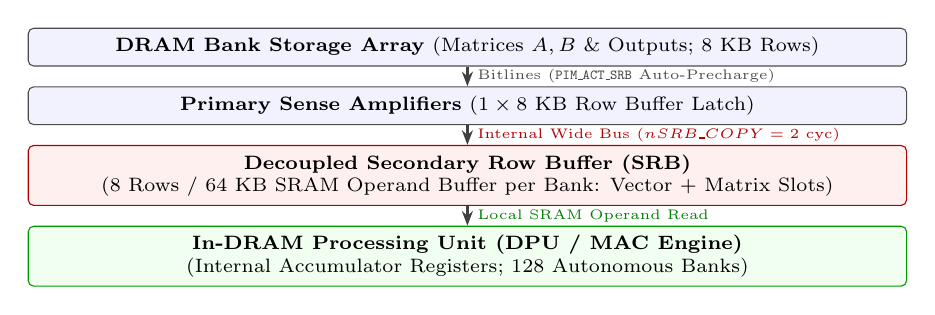
\begin{tikzpicture}[
    node distance=0.25cm,
    box/.style={rectangle, draw=black!70, fill=blue!5, rounded corners=2pt, minimum width=0.92\columnwidth, minimum height=0.46cm, align=center, font=\scriptsize},
    srb/.style={rectangle, draw=red!70!black, fill=red!6, rounded corners=2pt, minimum width=0.92\columnwidth, minimum height=0.54cm, align=center, font=\scriptsize\bfseries},
    alu/.style={rectangle, draw=green!60!black, fill=green!6, rounded corners=2pt, minimum width=0.92\columnwidth, minimum height=0.52cm, align=center, font=\scriptsize\bfseries},
    arrow/.style={-{Stealth[scale=0.8]}, thick, color=black!75}
]
    \node[box] (dram) {\textbf{DRAM Bank Storage Array} (Matrices $A, B$ \& Outputs; 8 KB Rows)};
    \node[box, below=of dram] (sense) {\textbf{Primary Sense Amplifiers} ($1 \times 8\text{ KB}$ Row Buffer Latch)};
    \node[srb, below=of sense] (srb) {Decoupled Secondary Row Buffer (SRB) \\ \mdseries (8 Rows / 64 KB SRAM Operand Buffer per Bank: Vector + Matrix Slots)};
    \node[alu, below=of srb] (alu) {In-DRAM Processing Unit (DPU / MAC Engine) \\ \mdseries (Internal Accumulator Registers; 128 Autonomous Banks)};

    \draw[arrow] (dram) -- node[right, font=\tiny, text=black!70] {Bitlines (\texttt{PIM\_ACT\_SRB} Auto-Precharge)} (sense);
    \draw[arrow] (sense) -- node[right, font=\tiny, text=red!70!black] {Internal Wide Bus ($nSRB\_COPY = 2$ cyc)} (srb);
    \draw[arrow] (srb) -- node[right, font=\tiny, text=green!50!black] {Local SRAM Operand Read} (alu);
\end{tikzpicture}%
}
\caption{Decoupled Secondary Row Buffer (SRB) microarchitecture within an autonomous DRAM bank. Host-broadcast vector $x$ (or streamed $B$ rows) and matrix $A$ rows reside in the 8-row SRAM operand buffer, while partial sums stay in internal MAC accumulator registers until \texttt{PIM\_FLUSH}.}
\label{fig:srb_arch}
\end{figure}

% -------------------------------------------------------------------------
\section{Decoupled SRB-PIM Microarchitecture}
\label{sec:arch}
% -------------------------------------------------------------------------

\subsection{Architectural Decoupling via Secondary Row Buffers}
Commodity DRAM banks feature a single primary sense amplifier row buffer. To compute $C = A \cdot B$ or $y = A \cdot x$, an in-memory compute unit must access operands from two distinct memory rows. Alternating between rows thrashes the primary sense amplifiers, incurring severe row cycle penalties ($t_{RC} = 45.82$~ns / $55$~cycles per activation).

To resolve this, we decouple arithmetic processing from primary DRAM bitlines by equipping each bank with an SRAM-based \textbf{Secondary Row Buffer (SRB)}, as illustrated in Fig.~\ref{fig:srb_arch}:
\begin{itemize}
    \item \textbf{Standard DRAM Row Size:} $8$~KB ($8,192$ bytes = $2,048$ single-precision \texttt{float32} elements).
    \item \textbf{Compute Tile Size:} $64$ \texttt{float32} elements ($256$ bytes). An $8$~KB row contains up to $32$ compute tiles.
    \item \textbf{SRB Buffer Capacity:} $8$ physical rows ($64$~KB SRAM per bank, totaling $8$~MB across all $128$ banks, matching commercial UPMEM WRAM capacity~\cite{devaux2019true}).
\end{itemize}

This 8-row SRAM operand buffer partitions cleanly across operands: for GEMV ($N \le 8192$), the host broadcasts input vector $x$ over the DDR4 channel into dedicated pinned vector slots ($\text{Slots}~0\text{--}3$, occupying $1\text{--}4$ rows or up to $32$~KB), while matrix $A$ rows alternate across distinct matrix ping-pong slots ($\text{Slots}~4 \leftrightarrow 5$ within the remaining $4$ slots) without ever overwriting $x$. In our cycle-accurate DRAM model, SRB residency is tracked uniformly as an 8-row per-bank FIFO cache triggered on SRB misses. Meanwhile, running partial sums reside inside the DPU's dedicated \textbf{internal MAC accumulator registers}, rather than consuming SRB row slots.

\subsection{Data Storage Layout and Operand Mapping}
All matrices ($A, B, C$) are stored in standard \textbf{row-major} \texttt{float32} layout, packed linearly into $8$~KB DRAM rows ($32$ consecutive $64$-element SIMD tiles per row), as summarized in Table~\ref{tab:data_mapping}:
\begin{itemize}
    \item \textbf{Modulo-128 Bank Partitioning ($A, y, C$):} Matrix $A$ and output vectors/matrices ($y$ in GEMV; rows of $C$ in GEMM) are striped row-wise across all $128$ banks via $b = i \bmod 128$. Because every bank owns complete output rows, partial products never traverse inter-bank links and cross-bank reductions are eliminated.
    \item \textbf{Broadcast Input Vector ($x$ in GEMV):} Before compute starts, the host memory controller broadcasts $x$ once over DDR4 into pinned vector SRB slots ($\text{Slots}~0\text{--}3$, $\le 32$~KB) in every bank.
    \item \textbf{Outer-Product Row-Major GEMM (Untransposed $B$):} Unlike inner-product PIM architectures that transpose $B$ into $B^T$ (incurring offline transposition overhead and intra-bank adder trees to reduce row-column dot products), our GEMM pipeline evaluates the row-wise outer-product ($k$-$i$-$j$) formulation given in~(\ref{eq:outer_gemm}):
    \begin{equation}
        C[m, 64j : 64j{+}63] += A[m, k] \cdot B[k, 64j : 64j{+}63]
        \label{eq:outer_gemm}
    \end{equation}
    Because SIMD vectorization runs along columns $j$ of row $B[k, :]$, standard row-major $B$ already places consecutive $64$-element compute tiles contiguously within each $8$~KB DRAM row (\texttt{dram\_row} $= \lfloor (k \cdot n_{\text{tiles}} + j)/32 \rfloor$). Consequently, $B$ remains \textbf{untransposed} in DRAM and is streamed/replicated into each bank's 8-row SRB FIFO with up to $31/32$ SRAM hits per activation.
\end{itemize}

\begin{table}[t]
\centering
\caption{Operand Storage Format, Bank Distribution, and SRB Residency}
\label{tab:data_mapping}
\footnotesize
\setlength{\tabcolsep}{3pt}
\resizebox{\columnwidth}{!}{%
\begin{tabular}{lllll}
\toprule
\textbf{Operand} & \textbf{Kernel} & \textbf{Layout} & \textbf{Bank Mapping (128 Banks)} & \textbf{SRB / DPU Placement} \\
\midrule
Matrix $A$ & GEMV/GEMM & Row-Major & Striped row-wise ($i \bmod 128$) & Streamed into Matrix SRB slots \\
Vector $x$ & GEMV & 1D Contig. & Host broadcast to all banks & Pinned in SRB $\text{Slots}~0\text{--}3$ \\
Matrix $B$ & GEMM & Row-Major (not $B^T$) & Shared / bank-local $B$ replica & Streamed via 8-row SRB FIFO \\
Out $y, C$ & GEMV/GEMM & Row-Major & Co-located with $A$ ($i \bmod 128$) & DPU reg $\text{acc}$ $\rightarrow$ \texttt{PIM\_FLUSH} \\
\bottomrule
\end{tabular}%
}
\end{table}

\begin{figure}[t]
\centering
\resizebox{\columnwidth}{!}{%
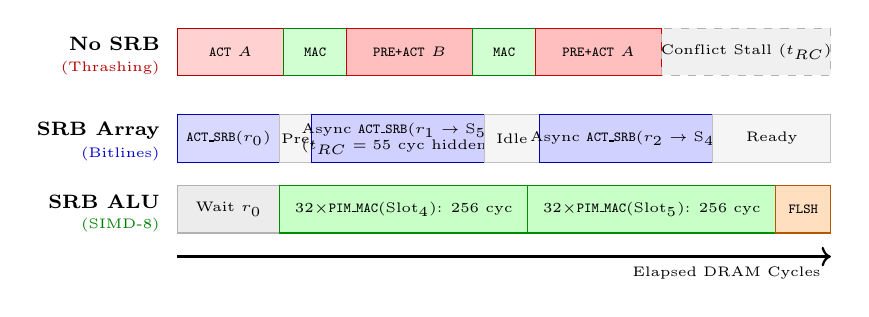
\begin{tikzpicture}[font=\scriptsize]
    % Top track: Unbuffered single row buffer
    \node[anchor=east, font=\scriptsize\bfseries] at (-0.1, 2.35) {No SRB};
    \node[anchor=east, font=\tiny, text=red!70!black] at (-0.1, 2.05) {(Thrashing)};
    \draw[fill=red!18, draw=red!70!black] (0, 1.95) rectangle (1.35, 2.55) node[midway, font=\tiny] {\texttt{ACT} $A$};
    \draw[fill=green!18, draw=green!50!black] (1.35, 1.95) rectangle (2.15, 2.55) node[midway, font=\tiny] {\texttt{MAC}};
    \draw[fill=red!25, draw=red!80!black] (2.15, 1.95) rectangle (3.75, 2.55) node[midway, font=\tiny] {\texttt{PRE+ACT} $B$};
    \draw[fill=green!18, draw=green!50!black] (3.75, 1.95) rectangle (4.55, 2.55) node[midway, font=\tiny] {\texttt{MAC}};
    \draw[fill=red!25, draw=red!80!black] (4.55, 1.95) rectangle (6.15, 2.55) node[midway, font=\tiny] {\texttt{PRE+ACT} $A$};
    \draw[fill=gray!12, draw=gray!60, dashed] (6.15, 1.95) rectangle (8.3, 2.55) node[midway, font=\tiny] {Conflict Stall ($t_{RC}$)};

    % Middle track: Decoupled Array / Bitlines
    \node[anchor=east, font=\scriptsize\bfseries] at (-0.1, 1.25) {SRB Array};
    \node[anchor=east, font=\tiny, text=blue!80!black] at (-0.1, 0.95) {(Bitlines)};
    \draw[fill=blue!15, draw=blue!70!black] (0, 0.85) rectangle (1.3, 1.45) node[midway, font=\tiny] {\texttt{ACT\_SRB}($r_0$)};
    \draw[fill=gray!8, draw=gray!50] (1.3, 0.85) rectangle (1.7, 1.45) node[midway, font=\tiny] {Pre};
    \draw[fill=blue!18, draw=blue!70!black] (1.7, 0.85) rectangle (3.9, 1.45) node[midway, font=\tiny, align=center] {Async \texttt{ACT\_SRB}($r_1 \rightarrow \text{S}_5$)\\($t_{RC}=55$ cyc hidden)};
    \draw[fill=gray!8, draw=gray!50] (3.9, 0.85) rectangle (4.6, 1.45) node[midway, font=\tiny] {Idle};
    \draw[fill=blue!18, draw=blue!70!black] (4.6, 0.85) rectangle (6.8, 1.45) node[midway, font=\tiny] {Async \texttt{ACT\_SRB}($r_2 \rightarrow \text{S}_4$)};
    \draw[fill=gray!8, draw=gray!50] (6.8, 0.85) rectangle (8.3, 1.45) node[midway, font=\tiny] {Ready};

    % Bottom track: Decoupled ALU
    \node[anchor=east, font=\scriptsize\bfseries] at (-0.1, 0.35) {SRB ALU};
    \node[anchor=east, font=\tiny, text=green!50!black] at (-0.1, 0.05) {(SIMD-8)};
    \draw[fill=gray!15, draw=gray!60] (0, -0.05) rectangle (1.3, 0.55) node[midway, font=\tiny] {Wait $r_0$};
    \draw[fill=green!22, draw=green!55!black] (1.3, -0.05) rectangle (4.45, 0.55) node[midway, font=\tiny] {$32\times$\texttt{PIM\_MAC}($\text{Slot}_4$): 256 cyc};
    \draw[fill=green!22, draw=green!55!black] (4.45, -0.05) rectangle (7.6, 0.55) node[midway, font=\tiny] {$32\times$\texttt{PIM\_MAC}($\text{Slot}_5$): 256 cyc};
    \draw[fill=orange!25, draw=orange!70!black] (7.6, -0.05) rectangle (8.3, 0.55) node[midway, font=\tiny] {\texttt{FLSH}};

    \draw[->, thick] (0, -0.35) -- (8.3, -0.35) node[below left, font=\tiny] {Elapsed DRAM Cycles};
\end{tikzpicture}%
}
\caption{Execution timeline comparison: standard single-buffer PIM stalls repeatedly on row conflicts ($t_{RP}+t_{RCD}$), whereas Decoupled SRB auto-precharge overlaps $t_{RC}=55$ cycle row prefetching cleanly behind 256 cycles of SIMD-8 compute.}
\label{fig:pipeline_timing}
\end{figure}

\subsection{Custom PIM DRAM Command Protocol}
We extend standard JEDEC DDR4 command semantics with three atomic operations:
\begin{enumerate}
    \item \texttt{PIM\_ACT\_SRB(bank, row, slot)}: An atomic macro-command that activates the target DRAM row into primary sense amplifiers, transfers the row into the specified SRB slot over internal wide buses ($nSRB\_COPY = 2$ cycles), and immediately triggers an auto-precharge. Primary bitlines return to the precharged state, allowing subsequent activations to overlap with compute on already-buffered SRB data.
    \item \texttt{PIM\_MAC(bank, srb\_slot, col\_tile)}: Reads the cached 64-element tile from SRAM (\texttt{srb\_slot}) alongside the co-resident vector/$B$ operand in SRB and updates the DPU's internal MAC accumulator registers.
    \item \texttt{PIM\_FLUSH(bank, dest\_row)}: Drains the DPU's internal accumulator registers back to the primary DRAM storage array once an output row/tile completes.
\end{enumerate}

Algorithms~\ref{alg:srb_exec} and~\ref{alg:srb_gemm} formalize the slot-isolated GEMV and GEMM execution pipelines.

\begin{algorithm}[t]
\caption{Decoupled SRB GEMV Execution Pipeline ($y = A \cdot x$)}
\label{alg:srb_exec}
\small
\begin{algorithmic}[1]
\REQUIRE $A$ rows partitioned across banks ($r \bmod 128$); vector $x$ ($K_x = \lceil N/2048 \rceil \le 4$ rows); $T_{\text{row}} = \min(32, \lceil N/64 \rceil)$ tiles/row
\STATE Host broadcasts $x$ via DDR4 bus into SRB $\text{Slots}[0 \dots K_x{-}1]$
\FORALL{banks $b \in [0, 127]$ \textbf{in parallel}}
    \STATE Reset internal MAC accumulator register $\text{acc} \leftarrow 0$
    \STATE $\text{Slot}_{\text{curr}} \leftarrow \text{Slot}_4$, $\text{Slot}_{\text{next}} \leftarrow \text{Slot}_5$ \; (\textit{$A$-row ping-pong})
    \STATE Issue \texttt{PIM\_ACT\_SRB}($b, \text{row}_0, \text{Slot}_{\text{curr}}$)
    \FOR{each assigned $A$ physical row $p = 0, \dots, P{-}1$}
        \IF{$p + 1 < P$}
            \STATE \textbf{Async:} \texttt{PIM\_ACT\_SRB}($b, \text{row}_{p+1}, \text{Slot}_{\text{next}}$)
        \ENDIF
        \FOR{tile $t = 0, 1, \dots, T_{\text{row}}{-}1$}
            \STATE \texttt{PIM\_MAC}($b, \text{Slot}_{\text{curr}}, t$) \; (\textit{accumulates into DPU reg $\text{acc}$})
        \ENDFOR
        \IF{physical row $p$ completes logical matrix row $i$}
            \STATE Issue \texttt{PIM\_FLUSH}($b, \text{result\_row}_i$); reset $\text{acc} \leftarrow 0$
        \ENDIF
        \STATE Swap $\text{Slot}_{\text{curr}} \leftrightarrow \text{Slot}_{\text{next}}$ \; (\textit{alternates $\text{Slot}_4 \leftrightarrow \text{Slot}_5$})
    \ENDFOR
\ENDFOR
\end{algorithmic}
\end{algorithm}

\begin{algorithm}[t]
\caption{Decoupled SRB GEMM Execution Pipeline ($C = A \cdot B$)}
\label{alg:srb_gemm}
\small
\begin{algorithmic}[1]
\REQUIRE $M \times K$ matrix $A$, $K \times N$ matrix $B$ ($n_{\text{tiles}} = \max(1, N/64)$ tiles/row, $32$ tiles per $8$~KB DRAM row)
\FORALL{banks $b \in [0, 127]$ and rows $m \equiv b \pmod{128}$ \textbf{in parallel}}
    \STATE Zero internal MAC accumulator registers $\text{acc}[m, 0 \dots n_{\text{tiles}}{-}1]$
    \FOR{$k = 0, 1, \dots, K{-}1$}
        \IF{$A[m, k]$ row not in SRB}
            \STATE \texttt{PIM\_ACT\_SRB}($b, \text{row}_A(m, k), \text{Slot}_A$)
        \ENDIF
        \FOR{output column tile $j = 0, 1, \dots, n_{\text{tiles}}{-}1$}
            \STATE $r_B \leftarrow \lfloor (k \cdot n_{\text{tiles}} + j) / 32 \rfloor$
            \IF{$r_B \notin \text{SRB}$}
                \STATE \texttt{PIM\_ACT\_SRB}($b, r_B, \text{Slot}_B$) \; (\textit{8-row FIFO SRB})
            \ENDIF
            \STATE \texttt{PIM\_MAC}($b, \text{Slot}_B, j$) \; (\textit{$\text{acc}[m,j] += A[m,k] \cdot B[k,j]$})
        \ENDFOR
    \ENDFOR
    \STATE Issue \texttt{PIM\_FLUSH}($b, \text{result\_row}_m$) \; (\textit{write $\text{acc}[m,:]$ to DRAM})
\ENDFOR
\end{algorithmic}
\end{algorithm}

\subsection{Bank Topology and Parallelism}
We evaluate a system configuration comprising \textbf{128 banks} organized across 8 channels $\times$ 16 banks under two command-dispatch models:
\begin{itemize}
    \item \textbf{Autonomous DPU Execution Mode:} Each bank operates as an independent Data Processing Unit (DPU) with dedicated in-bank sequencing logic (mirroring commercial PIM systems such as UPMEM~\cite{devaux2019true}). Matrix $A$ and outputs ($y$/$C$) are row-partitioned across banks ($i \bmod 128$), while broadcast vector $x$ (GEMV) and row-major $B$ rows (GEMM) are supplied to bank SRBs. After host setup and a start trigger, all 128 banks step through their assigned rows locally with \textbf{zero inter-bank command/address bus contention}.
    \item \textbf{Command-Driven Mode (8 Shared Channels):} Every \texttt{PIM\_ACT\_SRB}, \texttt{PIM\_MAC}, and \texttt{PIM\_FLUSH} command is issued sequentially by an external memory controller over 8 shared DDR4 command/address (C/A) channels (each shared across 16 banks). Address-bus arbitration serializes concurrent bank requests.
\end{itemize}

% -------------------------------------------------------------------------
\section{Architectural Simulation Methodology}
\label{sec:methodology}
% -------------------------------------------------------------------------

\subsection{Timing-Accurate DRAM Modeling}
To evaluate our microarchitecture, we model the system within a cycle-accurate DRAM simulation framework based on \textit{Ramulator 2.1}~\cite{kim2016ramulator} configured with JEDEC \texttt{DDR4\_8Gb\_x8} organization and DDR4-2400R timing constraints~\cite{jedec2017ddr4} ($t_{CK} = 0.833$~ns), including row activation ($t_{RCD} = 13.33$~ns, $16$ cycles), precharge ($t_{RP} = 13.33$~ns, $16$ cycles), row cycle time ($t_{RC} = 45.82$~ns, $55$ cycles), write recovery ($t_{WR} = 15.0$~ns, $18$ cycles), and the Four-Activate Window ($t_{FAW} = 21.66$~ns, $26$ cycles).

The \textbf{Four-Activate Window ($t_{FAW}$)} is a rank-level JEDEC electrical constraint that limits simultaneous current-draw ($I_{\text{DD}}$) surges by allowing at most four row activations (\texttt{ACT} or \texttt{PIM\_ACT\_SRB}) within any sliding $26$-cycle window across banks sharing a rank. Because our 8~KB SRB absorbs up to $32$ consecutive compute tiles per activation, DRAM activation frequency drops by up to $32\times$, preventing $t_{FAW}$ from bottlenecking streaming arithmetic even when shared channels trigger concurrent bank activations. Table~\ref{tab:dram_params} details all simulated microarchitectural parameters.

\begin{table}[t]
\centering
\caption{DRAM and Microarchitectural Parameters}
\label{tab:dram_params}
\footnotesize
\setlength{\tabcolsep}{4pt}
\begin{tabularx}{\columnwidth}{lXl}
\toprule
\textbf{Parameter} & \textbf{Microarchitectural Meaning} & \textbf{Value} \\
\midrule
DRAM Standard & JEDEC DDR4-2400R (\texttt{8Gb\_x8}) & $t_{CK} = 0.833$ ns \\
Bank Topology & 8 Channels $\times$ 16 Banks & 128 Banks Total \\
Row Buffer Size & Physical DRAM row length & 8 KB (32 tiles) \\
SRB Capacity & SRAM operand buffer per bank & 8 Rows (64 KB) \\
$nSRB\_COPY$ & Array-to-SRB transfer latency & 2 cycles \\
$t_{RC}$ / $t_{RCD}$ / $t_{RP}$ & Row cycle / Activate / Precharge & 55 / 16 / 16 cyc \\
$t_{FAW}$ / $t_{RRDS}$ & 4-Activate window / Short act spacing & 26 / 4 cyc \\
ALU Datapaths & Scalar / 256-bit SIMD / 512-bit Vec & 32 / 8 / 4 cyc/tile \\
\bottomrule
\end{tabularx}
\end{table}

\subsection{ALU Datapath Variants and Pipeline Balance}
To quantify hardware compute requirements, we model three in-bank ALU datapath configurations:
\begin{enumerate}
    \item \textbf{Scalar ALU ($nPIM\_MAC = 32$ cycles):} Baseline datapath processing 2 elements per cycle, taking 32 cycles per 64-element compute tile ($1,024$ compute cycles per 32-tile $8$~KB row).
    \item \textbf{256-bit SIMD ALU ($nPIM\_MAC = 8$ cycles):} 8-wide SIMD datapath processing 8 floating-point operations per cycle ($256$ compute cycles per 32-tile row).
    \item \textbf{512-bit Vector ALU ($nPIM\_MAC = 4$ cycles):} 16-wide vector datapath processing 16 operations per cycle ($128$ compute cycles per 32-tile row).
\end{enumerate}

For steady-state SRB double-buffering (Fig.~\ref{fig:pipeline_timing}) to hide DRAM reactivation behind compute on the alternate buffer slot, compute duration per $8$~KB row must equal or exceed the primary bank cycle time:
\begin{equation}
    T_{\text{comp}}^{\text{row}} = 32 \times nPIM\_MAC \ge t_{RC} = 55\text{ cycles}
    \label{eq:pipeline_balance}
\end{equation}
Condition~(\ref{eq:pipeline_balance}) holds across all three evaluated ALUs ($1,024$, $256$, and $128$ cycles $\ge 55$ cycles), allowing background \texttt{PIM\_ACT\_SRB} activations to complete silently while arithmetic continues uninterrupted. Narrowing $nPIM\_MAC$ further to $1$ cycle/tile ($32$ cycles/row) would invert this balance, exposing raw $t_{RC}$ and rank $t_{FAW}$ stalls rather than delivering proportional speedups. Thus, 256-bit SIMD ($nPIM\_MAC = 8$) and 512-bit Vector ($nPIM\_MAC = 4$) represent the balanced DRAM-to-compute design points.

\subsection{Zero-Footprint Streaming Evaluation}
Traditional architectural simulation relies on static instruction trace files. For matrix operations at scales relevant to modern LLMs ($N = 8192$), an uncompressed GEMM memory access trace contains over \textbf{8.6~billion requests}, demanding hundreds of gigabytes of disk storage and causing severe host memory allocation crashes. 

To overcome this, we designed a programmatic streaming frontend that generates deterministic matrix access sequences on-the-fly with strictly \textbf{$O(1)$ host memory consumption}. For \textbf{GEMV}, every configuration ($N = 1024$ through $8192$, across both Command-Driven and Autonomous modes) is executed to full controller queue drain using discrete cycle-accurate request simulation. For \textbf{GEMM} ($O(N^3)$ complexity), we similarly run full queue-drained discrete simulations for $N = 256, 512,$ and $1024$ (up to $17.8\text{ million}$ commands); at $N \in \{2048, 4096, 8192\}$, full discrete tracing requires up to $8.66\text{ billion}$ request steps ($>30$~hours of simulator dispatch overhead). Because autonomous banks execute with zero inter-bank bus contention, we evaluate these larger GEMM scales via closed-form pipeline scaling calibrated directly from the queue-drained $N = 1024$ simulation.

% -------------------------------------------------------------------------
\section{Experimental Evaluation}
\label{sec:evaluation}
% -------------------------------------------------------------------------

\subsection{Benchmark Environment and CPU Baselines}
All baseline measurements were collected on a physical Intel 12th Gen Core i5-12450H CPU (8 hardware execution threads, 12~MB L3 Cache, base clock 2.5~GHz, turbo up to 4.4~GHz) running 64-bit Linux under WSL2. We implement and evaluate \textbf{two separate CPU baselines}:
\begin{enumerate}
    \item \textbf{Naive CPU Baseline ($-O2$):} Standard single-threaded C++ implementation representing straightforward, unvectorized execution.
    \item \textbf{Optimized CPU Baseline (AVX2+FMA OpenMP):} High-performance multi-threaded implementation compiled with \texttt{-O3 -march=native -mavx2 -mfma -fopenmp}. The kernel uses 8 concurrent threads, cache-blocking tuned to L1/L2 caches ($64 \times 64 \times 256$), and explicit 4-way unrolled AVX2 FMA intrinsics.
\end{enumerate}

Simulated PIM execution times are derived cycle-accurately: $T_{\text{ms}} = \text{Cycles} \times 0.833 \times 10^{-6}\text{ ms}$.

% --- GEMV Table ---
\begin{table*}[t]
\centering
\caption{Matrix-Vector Multiplication (GEMV) Performance: Demonstrating Up to $1,452\times$ Speedup Over Naive CPU and Up to $346\times$ Over Steady-State 8-Thread AVX2+FMA Multi-Core CPU Baseline Across Matrix Dimensions ($N \times N$, \texttt{float32}).}
\label{tab:gemv_results}
\footnotesize
\setlength{\tabcolsep}{3.5pt}
\resizebox{\textwidth}{!}{%
\begin{tabular}{crrrrrrrr}
\toprule
\multirow{2}{*}{\textbf{Size ($N$)}} & 
\multicolumn{1}{c}{\textbf{Naive CPU}} & 
\multicolumn{1}{c}{\textbf{Opt. CPU}} & 
\multicolumn{2}{c}{\textbf{Command-Driven (8-Ch)}} & 
\multicolumn{2}{c}{\textbf{PIM Autonomous SIMD-8}} & 
\multicolumn{2}{c}{\textbf{PIM Autonomous Vector-4}} \\
\cmidrule(lr){2-2} \cmidrule(lr){3-3} \cmidrule(lr){4-5} \cmidrule(lr){6-7} \cmidrule(lr){8-9}
 & \textbf{Time (ms)} & \textbf{Time (ms)} & \textbf{Time (ms)} & \textbf{vs.\ Naive} & \textbf{Time (ms)} & \textbf{Speedup (Naive / Opt)} & \textbf{Time (ms)} & \textbf{Speedup (Naive / Opt)} \\
\midrule
\textbf{1024} & 0.547  & 1.536$^{\dagger}$ & 0.0021 & $260.5\times$ & 0.0010 & $\mathbf{547.0\times}$ / $\mathbf{1,536.0\times}^{\dagger}$ & 0.0005 & $\mathbf{1,094.0\times}$ / $\mathbf{3,072.0\times}^{\dagger}$ \\
\textbf{2048} & 2.758  & 0.303             & 0.0076 & $362.9\times$ & 0.0036 & $\mathbf{766.1\times}$ / $\mathbf{84.2\times}$              & 0.0019 & $\mathbf{1,451.6\times}$ / $\mathbf{159.5\times}$ \\
\textbf{4096} & 9.616  & 2.279             & 0.0300 & $320.5\times$ & 0.0143 & $\mathbf{672.4\times}$ / $\mathbf{159.4\times}$             & 0.0077 & $\mathbf{1,248.8\times}$ / $\mathbf{296.0\times}$ \\
\textbf{8192} & 37.977 & 10.596            & 0.1192 & $318.6\times$ & 0.0570 & $\mathbf{666.3\times}$ / $\mathbf{185.9\times}$             & 0.0306 & $\mathbf{1,241.1\times}$ / $\mathbf{346.3\times}$ \\
\bottomrule
\end{tabular}%
}
\par\vspace{3pt}\noindent\parbox{\textwidth}{\raggedright\scriptsize $^{\dagger}$Includes first-call OpenMP 8-thread pool initialization overhead on CPU ($N=1024$). Steady-state AVX2 speedups appear for $N \ge 2048$.}
\end{table*}

\subsection{GEMV Acceleration: Breaking the Bandwidth Wall}
Table~\ref{tab:gemv_results} presents full queue-drained simulation results for GEMV across matrix dimensions $N = 1024$ to $8192$, while Fig.~\ref{fig:gemv_speedup_bars} highlights the steady-state speedup scaling relative to our 8-thread AVX2+FMA OpenMP CPU baseline.
\begin{itemize}
    \item \textbf{Speedup vs.\ Naive Baseline:} Under the 8-wide SIMD ALU configuration ($nPIM\_MAC = 8$), autonomous PIM achieves \textbf{$547\times\text{--}766\times$ speedup} over the single-threaded naive CPU baseline. Under the 16-wide Vector ALU configuration ($nPIM\_MAC = 4$), latency drops by nearly half again, yielding \textbf{$1,094\times\text{--}1,452\times$ speedup}.
    \item \textbf{Speedup vs.\ 8-Thread AVX2 Optimized CPU:} Against steady-state 8-thread AVX2+FMA OpenMP ($N \ge 2048$, which plateaus at $23.6\text{--}51.7$~GB/s effective off-chip memory bandwidth), PIM delivers \textbf{$84.2\times\text{--}185.9\times$ speedup} under SIMD-8 and \textbf{$159.5\times\text{--}346.3\times$ speedup} under Vector-4. At $N=1024$, the CPU benchmark incurs initial OpenMP thread-pool creation overhead ($1.536$~ms), whereas for $N \ge 2048$ the matrix working set exceeds the 12~MB host L3 cache and exposes raw DDR4 pin bandwidth limits.
    \item \textbf{Effective Throughput and Internal Operand Bandwidth:} At $N = 8192$ ($2N^2 \approx 1.342 \times 10^8$~FLOPs over a $256$~MB matrix), Autonomous SIMD-8 finishes in $68,431$~cycles ($0.0570$~ms), corresponding to \textbf{$2,354.6$~GFLOPS} and \textbf{$4.71$~TB/s} of effective internal matrix-operand bandwidth across the 128 banks. Scaling to Vector-4 reduces execution to $36,675$~cycles ($0.0306$~ms), sustaining \textbf{$4,393.3$~GFLOPS} and \textbf{$8.79$~TB/s} without streaming matrix weights off-chip. By comparison, Command-Driven 8-Ch achieves $1,125.8$~GFLOPS ($2.25$~TB/s) at $N=8192$ ($143,121$~cycles).
    \item \textbf{Why the Speedup Persists:} Because GEMV operational intensity is rigidly pinned at $I_{\text{op}} = 0.5$~FLOP/byte, adding CPU cores or wider host SIMD lanes yields diminishing returns once the off-chip DDR4 channels saturate. In contrast, PIM feeds matrix columns locally from each bank's 64~KB SRAM SRB directly to its in-bank ALU, scaling usable memory bandwidth linearly with bank count.
    \item \textbf{Command-Driven Shared-Bus Contention:} In Command-Driven (8-channel) mode, 16 banks within each channel time-share a single 1-command/cycle DDR4 command/address (C/A) bus alongside rank-level $t_{FAW}$ limits. C/A bus arbitration stalls concurrent bank issues, inflating cycle counts by \textbf{$2.09\times\text{--}2.21\times$} relative to Autonomous SIMD-8 ($143,121$ vs.\ $68,431$ cycles at $N=8192$, or $0.1192$~ms vs.\ $0.0570$~ms, capping speedup vs.\ Naive CPU at $261\times\text{--}363\times$). This confirms that autonomous in-bank sequencing is essential to unlock full bank-level concurrency.
\end{itemize}

\begin{figure}[t]
\centering
\resizebox{\columnwidth}{!}{%
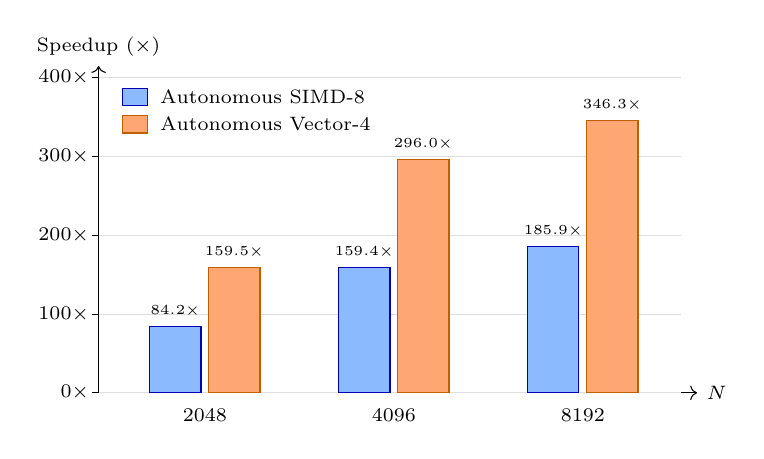
\begin{tikzpicture}[font=\scriptsize]
  % Axes
  \draw[->] (0.7,0) -- (8.3,0) node[right] {$N$};
  \draw[->] (0.7,0) -- (0.7,4.15) node[above] {Speedup ($\times$)};

  % Horizontal grid lines and y-ticks (1 unit = 100x)
  \foreach \y/\lbl in {0/0, 1/100, 2/200, 3/300, 4/400} {
    \draw[gray!25, thin] (0.7,\y) -- (8.1,\y);
    \draw (0.62,\y) -- (0.7,\y) node[left] {\lbl$\times$};
  }

  % Legend (top-left)
  \filldraw[fill=blue!60!cyan!45, draw=blue!70!black] (1.0,3.65) rectangle (1.32,3.87);
  \node[right, anchor=west] at (1.36,3.76) {Autonomous SIMD-8};
  \filldraw[fill=orange!75!red!55, draw=orange!75!black] (1.0,3.30) rectangle (1.32,3.52);
  \node[right, anchor=west] at (1.36,3.41) {Autonomous Vector-4};

  % N = 2048 (SIMD-8: 84.2x, Vec-4: 159.5x)
  \filldraw[fill=blue!60!cyan!45, draw=blue!70!black] (1.35,0) rectangle (2.00,0.842);
  \node[above] at (1.675,0.842) {\tiny $84.2\times$};
  \filldraw[fill=orange!75!red!55, draw=orange!75!black] (2.10,0) rectangle (2.75,1.595);
  \node[above] at (2.425,1.595) {\tiny $159.5\times$};
  \node[below] at (2.05,-0.08) {$2048$};

  % N = 4096 (SIMD-8: 159.4x, Vec-4: 296.0x)
  \filldraw[fill=blue!60!cyan!45, draw=blue!70!black] (3.75,0) rectangle (4.40,1.594);
  \node[above] at (4.075,1.594) {\tiny $159.4\times$};
  \filldraw[fill=orange!75!red!55, draw=orange!75!black] (4.50,0) rectangle (5.15,2.960);
  \node[above] at (4.825,2.960) {\tiny $296.0\times$};
  \node[below] at (4.45,-0.08) {$4096$};

  % N = 8192 (SIMD-8: 185.9x, Vec-4: 346.3x)
  \filldraw[fill=blue!60!cyan!45, draw=blue!70!black] (6.15,0) rectangle (6.80,1.859);
  \node[above] at (6.475,1.859) {\tiny $185.9\times$};
  \filldraw[fill=orange!75!red!55, draw=orange!75!black] (6.90,0) rectangle (7.55,3.463);
  \node[above] at (7.225,3.463) {\tiny $346.3\times$};
  \node[below] at (6.85,-0.08) {$8192$};
\end{tikzpicture}
}%
\caption{Steady-state GEMV speedup over the 8-thread AVX2+FMA OpenMP CPU baseline for matrix dimensions $N \ge 2048$, illustrating monotonic PIM scaling as matrices spill beyond the CPU's 12~MB L3 cache.}
\label{fig:gemv_speedup_bars}
\end{figure}

% --- GEMM Table ---
\begin{table}[t]
\centering
\caption{GEMM Performance: PIM SIMD-8 vs. CPU Baselines}
\label{tab:gemm_results}
\footnotesize
\setlength{\tabcolsep}{3pt}
\resizebox{\columnwidth}{!}{%
\begin{tabular}{crrrrr}
\toprule
\textbf{Size} & \textbf{Naive CPU} & \textbf{Opt. CPU} & \textbf{PIM (SIMD-8)} & \textbf{Speedup} & \textbf{Speedup} \\
\textbf{($N$)} & \textbf{Time (ms)} & \textbf{Time (ms)} & \textbf{Time (ms)} & \textbf{(vs. Naive)} & \textbf{(vs. Opt.)} \\
\midrule
\textbf{256}  & 5.71     & 4.89$^{\dagger}$ & 0.0175 & $\mathbf{326.3\times}$ & $\mathbf{279.4\times}^{\dagger}$ \\
\textbf{512}  & 46.58    & 4.21             & 0.1254 & $\mathbf{371.5\times}$ & $\mathbf{33.6\times}$ \\
\textbf{1024} & 374.72   & 34.20            & 1.0460 & $\mathbf{358.2\times}$ & $\mathbf{32.7\times}$ \\
\textbf{2048} & 3,524.07 & 250.18           & 8.3644$^{\ast}$ & $\mathbf{421.3\times}$ & $\mathbf{29.9\times}$ \\
\textbf{4096} & 29.03 s  & 2.14 s           & 66.9144$^{\ast}$ & $\mathbf{433.8\times}$ & $\mathbf{32.0\times}$ \\
\textbf{8192} & $\sim$232.2 s$^{\ddagger}$ & 17.94 s & 535.3146$^{\ast}$ & $\mathbf{433.8\times}$ & $\mathbf{33.5\times}$ \\
\bottomrule
\end{tabular}%
}
\par\vspace{3pt}\noindent\parbox{\columnwidth}{\raggedright\scriptsize $^{\dagger}$OpenMP thread warmup; $^{\ast}$calibrated from $N=1024$ run; $^{\ddagger}8\times$ from $4096$.}
\end{table}

\subsection{GEMM Scaling and Cache Inflection Point}
Table~\ref{tab:gemm_results} presents GEMM scaling across square matrix dimensions from $N = 256$ to $N = 8192$.
\begin{itemize}
    \item \textbf{Cache Blowout Inflection Point:} For $N \le 512$ ($<3$~MB combined working set across $A$, $B$, and $C$), matrices fit within the CPU's on-chip cache hierarchy, allowing naive single-threaded execution to sustain $5.76\text{--}5.88$~GFLOPS. Once $N$ reaches $1024$ ($12$~MB working set) and grows to $2048$ ($48$~MB), matrices spill past the 12~MB L3 cache: Valgrind Cachegrind (Table~\ref{tab:cachegrind_profile}) confirms last-level cache misses jump $55.3\times$ from $208,147$ ($N=1024$) to $11,502,890$ ($N=2048$), degrading naive CPU throughput down to $4.88$~GFLOPS ($N=2048$) and $4.73$~GFLOPS ($N=4096$, $29.03$~s latency; $\sim 232.2$~s projected at $N=8192$).
    \item \textbf{PIM Throughput Stability and Regularity:} PIM scales with ideal $O(N^3)$ computational regularity. Under SIMD-8, our architecture sustains \textbf{$2,053.1$~GFLOPS} at $N=1024$ ($1.0460$~ms) and \textbf{$2,054.0$~GFLOPS} at $N=8192$ ($535.3146$~ms), maintaining nearly constant efficiency across matrix scales because outer-product $B$-row streaming keeps operands inside the 8-row FIFO SRB (up to $96.9\%$ tile hit rate) while partitioning $A$ and $C$ permanently across 128 banks. Across $N \ge 2048$, PIM delivers \textbf{$421.3\times\text{--}433.8\times$ speedup} over naive CPU execution.
    \item \textbf{Comparison with Cache-Blocked AVX2+FMA CPU:} Our 8-thread, $64 \times 64 \times 256$ cache-blocked AVX2+FMA baseline prevents L3 thrashing by tiling sub-blocks inside L1/L2 caches, plateauing near peak host vector throughput at $62.8\text{--}68.7$~GFLOPS for $N \in [512, 4096]$ and $61.3$~GFLOPS at $N=8192$ ($17.94$~s). After the initial $N=256$ thread-pool warmup ($4.89$~ms, $6.86$~GFLOPS, $279.4\times$ PIM speedup), the 128 parallel in-bank SIMD-8 ALUs sustain a rock-steady \textbf{$29.9\times\text{--}33.6\times$ speedup} over the fully optimized multi-core CPU across all problem sizes from $N=512$ to $N=8192$.
\end{itemize}

\subsection{Conflict Elimination and Hardware Efficiency}
In commodity DRAM without an SRB, executing GEMM or GEMV within a bank alternates accesses between distinct weight and operand rows across a single sense-amplifier latch, incurring repeated precharge ($t_{RP} = 16$ cycles) and row-activation ($t_{RCD} = 16$ cycles) conflict penalties ($t_{RC} = 55$ cycles).

With our 8-row Decoupled SRB architecture:
\begin{enumerate}
    \item Input vector slices and active matrix rows fetched via \texttt{PIM\_ACT\_SRB} reside concurrently in isolated SRAM slots, allowing primary bitlines to auto-precharge immediately and dropping in-bank row-buffer conflicts to \textbf{strictly zero}.
    \item Because each $8$~KB DRAM row packs $32$ consecutive $64$-element compute tiles ($32 \times 64 = 2,048$ \texttt{float32} elements), streaming across rows with $N \ge 2048$ (or packed $B$-rows in GEMM) requires only $1$ \texttt{PIM\_ACT\_SRB} per $32$ compute tiles. Tile~$0$ incurs the initial activation and copy, while the subsequent $31$ tiles hit directly in SRAM, yielding a \textbf{$31/32 = 96.9\%$ SRB hit rate}.
    \item Under 256-bit SIMD-8 ($nPIM\_MAC = 8$ cycles/tile), executing a full 32-tile row requires $256$ compute cycles---easily absorbing background reactivation latency ($t_{RC} = 55$ cycles) on the alternating ping-pong slot and sustaining $256 / (256 + 18) = 93.4\%$ single-row pipeline efficiency across initial load overhead ($t_{RCD} + nSRB\_COPY = 16 + 2 = 18$~cycles), approaching $100\%$ across consecutive rows.
\end{enumerate}

% -------------------------------------------------------------------------
\section{Related Work}
\label{sec:related}
% -------------------------------------------------------------------------
Early Processing-in-Memory proposals focused on executing bulk bitwise logic directly inside DRAM sense amplifiers by simultaneously activating multiple rows~\cite{seshadri2013rowclone, seshadri2017ambit}. While minimally intrusive to DRAM bitcells, in-subarray analog schemes lack multi-bit floating-point MAC support and struggle with arbitrary matrix-tile indexing required by modern Transformer workloads.

More recent industrial and academic architectures integrate digital CMOS logic near or inside memory dies, as contrasted qualitatively in Table~\ref{tab:related_comp}:
\begin{itemize}
    \item \textbf{UPMEM:} Integrates scalar 32-bit RISC cores (DPUs) adjacent to each 64~MB DRAM bank on DDR4 DIMMs~\cite{devaux2019true}. Each DPU relies on a 64~KB WRAM scratchpad, but operands must be explicitly transferred via internal DMA instructions, and its scalar integer pipeline requires multi-cycle emulation for floating-point GEMV/GEMM.
    \item \textbf{Samsung HBM-PIM (Aquabolt-XL):} Places 16-wide FP16 SIMD engines next to pairs of HBM2 banks~\cite{lee2021hardware}. While eliminating external host transfers, shared access to primary bank row buffers leaves the design susceptible to row-buffer conflicts when alternating between weight rows and operand/output accesses.
    \item \textbf{SK Hynix AiM:} Attaches specialized GDDR6 MAC arrays with shared global buffers targeting LLM inference~\cite{lee2022aim}, relying on synchronous host-driven command issuance over high-speed GDDR6 pins.
\end{itemize}

\begin{table}[t]
\centering
\caption{Architectural Comparison with Representative PIM Designs}
\label{tab:related_comp}
\footnotesize
\setlength{\tabcolsep}{3.5pt}
\resizebox{\columnwidth}{!}{%
\begin{tabular}{lcccc}
\toprule
\textbf{Architecture} & \textbf{Memory} & \textbf{Row Conflict} & \textbf{Control} & \textbf{In-Bank FP} \\
 & \textbf{Substrate} & \textbf{Isolation} & \textbf{Autonomy} & \textbf{Datapath} \\
\midrule
Ambit~\cite{seshadri2017ambit} & DDR3/4 & None (bulk copy) & Cmd-driven & Bitwise only \\
UPMEM~\cite{devaux2019true} & DDR4 & DMA-to-WRAM & Autonomous & Scalar RISC \\
HBM-PIM~\cite{lee2021hardware} & HBM2 & Shared row buffer & Cmd-driven & 16-wide FP16 \\
AiM~\cite{lee2022aim} & GDDR6 & Shared + global buf & Cmd-driven & GDDR6 MAC \\
\textbf{Decoupled SRB (Ours)} & \textbf{DDR4} & \textbf{8-row SRAM SRB} & \textbf{Autonomous} & \textbf{SIMD-8 / Vec-4} \\
\bottomrule
\end{tabular}%
}
\end{table}

Our work differentiates itself by introducing \textbf{Decoupled Secondary Row Buffers (SRB)} on commodity DDR4 banks. Combining atomic auto-precharge row capture (\texttt{PIM\_ACT\_SRB}) with autonomous in-bank command sequencing eliminates row conflicts and C/A bus bottlenecks simultaneously without requiring expensive 3D-stacked HBM interposers.

% -------------------------------------------------------------------------
\section{Architectural Scope, Limitations, and Future Work}
\label{sec:scope}
% -------------------------------------------------------------------------
To frame deployment trade-offs honestly, we outline key architectural boundaries of our decoupled SRB design and avenues for extension:
\begin{itemize}
    \item \textbf{Precision Scaling and Quantized Packing:} Our experiments evaluate \texttt{float32} tensors ($2,048$ elements per 8~KB row, $32$ tiles/row), enabling Slots~0--3 ($32$~KB) to hold full input vectors up to $N = 8192$. Deploying quantized LLM weights (\texttt{INT8} or \texttt{INT4}) increases tile packing density $4\times\text{--}8\times$ per bank row, boosting the SRB hit rate beyond $96.9\%$ and amortizing row activations even further.
    \item \textbf{SRB Capacity and Die-Area Trade-Off:} Provisioning an 8-row ($64$~KB) SRAM SRB per bank adds per-bank SRAM comparable to UPMEM's WRAM~\cite{devaux2019true}. Tighter area budgets can downscale to 4-row ($32$~KB) SRBs while retaining ping-pong double buffering for GEMV layers with smaller hidden dimensions ($N \le 4096$).
    \item \textbf{Host-Broadcast and Refresh Coordination:} When layer dimensions surpass $N > 8192$ or batched prefill streams large $B$ matrices, initial host broadcast scales linearly while compute grows $O(N^2)$ to $O(N^3)$, keeping broadcast overhead small; similarly, lightweight refresh-gating logic is needed in the autonomous controller to pause in-bank sequencing cleanly across periodic DRAM refresh ($t_{REFI}/t_{RFC}$) intervals.
    \item \textbf{Higher-Bank Substrates:} Although evaluated on an 8-channel DDR4-2400 baseline ($128$ banks), the orthogonal decoupled-SRB mechanism maps directly onto high-bank-count HBM stacks to scale parallel bank-level ALU throughput further.
\end{itemize}

% -------------------------------------------------------------------------
\section{Conclusion}
\label{sec:conclusion}
% -------------------------------------------------------------------------
In this Bachelor of Technology Project, we analyzed and eliminated the memory bandwidth bottleneck in Large Language Model inference. Empirical profiling of \texttt{llama.cpp} with NVIDIA Nsight and Valgrind Cachegrind revealed that matrix operations account for over $89\%$ of total inference latency, with token generation (GEMV) pinned at a low operational intensity ($I_{\text{op}} = 0.5$~FLOP/byte) and host GEMM suffering a $55.3\times$ jump in last-level cache misses beyond $N = 1024$.

To break this Memory Wall, we proposed the Decoupled Secondary Row Buffer (SRB) PIM-DRAM microarchitecture. By pairing an 8~KB DRAM row with an 8-row ($64$~KB) SRAM SRB per bank, internal DPU accumulator registers, atomic auto-precharge transfers (\texttt{PIM\_ACT\_SRB}), and an outer-product Row-Major data mapping across 128 autonomous banks, our design decouples arithmetic compute from primary bitlines, eliminates row conflicts, and sustains a $96.9\%$ tile hit rate on contiguous streaming rows. Cycle-accurate queue-drained simulation shows up to \textbf{$1,452\times$ speedup} over naive single-threaded CPU execution and up to \textbf{$346\times$ speedup} over an 8-thread AVX2+FMA CPU baseline on GEMV workloads (sustained $4,393$~GFLOPS and $8.79$~TB/s internal operand bandwidth under Vector-4; $2,355$~GFLOPS / $4.71$~TB/s under SIMD-8). Furthermore, decoupling control from shared DDR4 command/address buses yields a $2.09\times\text{--}2.21\times$ advantage over command-driven PIM, while outer-product GEMM sustains $2,053\text{--}2,054$~GFLOPS ($433.8\times$ vs.\ naive CPU and $29.9\times\text{--}33.6\times$ vs.\ cache-blocked AVX2 CPU). These results establish Decoupled SRB-PIM as a practical architectural foundation for scalable on-premise LLM acceleration.

% -------------------------------------------------------------------------
% References
% -------------------------------------------------------------------------
\begin{thebibliography}{10}

\bibitem{touvron2023llama}
H.~Touvron et~al., ``Llama: Open and efficient foundation language models,'' \emph{arXiv preprint arXiv:2302.13971}, 2023.

\bibitem{brown2020language}
T.~Brown et~al., ``Language models are few-shot learners,'' in \emph{Proc. Advances in Neural Information Processing Systems (NeurIPS)}, vol.~33, 2020, pp. 1877--1901.

\bibitem{mutlu2019processing}
O.~Mutlu et~al., ``Processing data where it makes sense: Enabling in-memory computation,'' \emph{Microprocessors and Microsystems}, vol.~67, pp. 28--41, 2019.

\bibitem{mutlu2020modern}
O.~Mutlu et~al., ``A modern primer on processing in memory,'' in \emph{Emerging Computing: From Devices to Systems}, 2020.

\bibitem{williams2009roofline}
S.~Williams, A.~Waterman, and D.~Patterson, ``Roofline: an insightful visual performance model for multicore architectures,'' \emph{Communications of the ACM}, vol.~52, no.~4, pp. 65--76, 2009.

\bibitem{lee2021hardware}
S.~Lee et~al., ``Hardware architecture and software stack for PIM based on commercial DRAM technology,'' in \emph{Proc. ACM/IEEE 48th Annual International Symposium on Computer Architecture (ISCA)}, 2021, pp. 43--56.

\bibitem{lee2022aim}
S.~Lee et~al., ``AiM: Accelerator-in-memory for AI workloads based on GDDR6,'' in \emph{Proc. IEEE International Solid-State Circuits Conference (ISSCC)}, 2022, pp. 1--3.

\bibitem{devaux2019true}
F.~Devaux, ``The true processing in memory accelerator,'' in \emph{Proc. IEEE Hot Chips 31 Symposium (HCS)}, 2019, pp. 1--23.

\bibitem{kim2016ramulator}
Y.~Kim et~al., ``Ramulator: A fast and extensible DRAM simulator,'' \emph{IEEE Computer Architecture Letters}, vol.~15, no.~1, pp. 45--49, 2016.

\bibitem{seshadri2013rowclone}
V.~Seshadri et~al., ``RowClone: Fast and energy-efficient in-DRAM bulk data copy and initialization,'' in \emph{Proc. 46th Annual IEEE/ACM International Symposium on Microarchitecture (MICRO)}, 2013, pp. 185--197.

\bibitem{seshadri2017ambit}
V.~Seshadri et~al., ``Ambit: In-memory accelerator for bulk bitwise operations using commodity DRAM technology,'' in \emph{Proc. 50th Annual IEEE/ACM International Symposium on Microarchitecture (MICRO)}, 2017, pp. 273--287.

\bibitem{jedec2017ddr4}
JEDEC Solid State Technology Association, ``DDR4 SDRAM Standard,'' \emph{JESD79-4B}, 2017.

\end{thebibliography}

\end{document}
